\section{Introduction}

There is humongous amount of data being produced and collected around us.
However, such large volumes of data needs to be processed to get meaningful insights.
Traditional Database systems cannot scale to such volumes of data.
Most shared memory based system would not scale for Petabytes of Data. 
Sharding can help but would not be viable option always. 
Most disk based systems on other hands need more expensive hardware as the data volume increases.
This has led to wide adoption of Big Data technologies everywhere and enterprises are moving their 
data to big data platforms. On the other hand SQL has been de-facto language of choice for 
data manipulation and data access. It is very popular data language among analysts, 
software engineers etc to query, manipulate and visualize data. Hence, it was only imminent that 
SQL would continue to be supported on big data platforms too. 
There are quite a few offerings that provide SQL on big data. There are commercial products like HAWQ and many open source products like Apache Hive, SparkSQL, Presto that provides SQL for big data. SQL workloads on big data can be classified broadly into following categories based on their usage:
\begin{description}
  \item[$\bullet$] ETL queries
  \item[$\bullet$] Reporting queries
  \item[$\bullet$] Ad-hoc queries
\end{description}

These technologies support running queries on structured, semi-structured data like JSON, XML etc and unstructured data. Some of the design goals of SQL on big data are following:
\begin{description}
  \item[$\bullet$] Cheap and horizontally scalable
  \item[$\bullet$] High Concurrency
  \item[$\bullet$] Low latency
\end{description}


SQL-on-Big Data has 3 layers which we have identified for optimizing SQL workloads:
\begin{description}
  \item[$\bullet$] Data Model:
  There are many aspects of Data Model that can be tuned to optimize Reporting or Ad-hoc queries.
  Historical queries can be analysed to recommend data formats for heavily used tables, recommend new partitions 
  or columns to sort on when tables are in columnar format. This is beyond the scope of this paper and we will not discuss about them in this work.
  \item[$\bullet$] Execution Engine:
  In this work we have evaluated popular SQL-on-Big Data tools like Apache Hive and SparkSQL. Apache Hive runs on underlying data processing engines like Hadoop MapReduce, Apache Tez or Apache Spark. SparkSQL runs on Spark. These query engines along with underlying data processing engine offer plethora of configuration parameters to tune. This is a challenging and time consuming task even for experts. As we have observed with large installations there can be thousands of queries being fired on daily basis and manual tuning the stack to cater to most of these queries is infeasible. Even the defaults for these configurations based on general rule of thumb can be way off from the optimal configuration for a particular workload. In this work we would present mathematical model using which this process can be automated for the ETL queries that run periodically. Our work would look at one run of these queries and use it to auto tune the configuration parameters.
  \item[$\bullet$] Cluster:
  Performance and the cost of the Big Data Stack is heavily sensitive to the Hardware configuration of the cluster of machines they run on. Especially when these installations are on Cloud there are many machine types available with different configurations. In this work we would be able to recommend machine type for a particular workload among the multiple options provided. 
\end{description}

\section{Related Work}
There are earlier works which have tried to optimize Hadoop workloads. These can broadly be classified into two categories:
\begin{description}
\item Mathematical Model Based
\item Actual Execution Based
\end{description}

\subsection{Mathematical Model Based}
Starfish was one of the first to model hadoop performance. In Starfish,
a component named \textit{What-if} engine estimated the cost of Hadoop Job using Simulation and
Hadoop Cost Model. The Cost-based optimizer (CBO) uses the what-if engine and recursive random search (RSS)
for tuning the parameters for a new Hadoop job. There were other works like Wu et al \cite{wu2013self} that followed Starfish. These methods collect information about the jobs executed on hadoop, a process
known as profiling. Job “signatures”, i.e., the resource utilization patterns of the jobs are used for profiling. In
the offline phase, using a training set, the jobs are clustered
(using variants of k-means) according to their respective signatures.
In the online phase [21] trains a SVM which makes
accurate and fast prediction of a job’s performance for various
configuration parameters and input data sizes. For any
new job, its signature is matched with the profiles of one
of the clusters, after which that cluster’s optimal parameter
configuration is used. In \cite{wu2013self} , the optimal parameter con-
figuration for every cluster is obtained through simulated
annealing, albeit for a reduced parameter search space.
An online MapReduce performance tuner (MROnline) is
developed in [22]. It is desgined and implemented on YARN
[30]. MROnline consists of a centralized master component which is the online tuner. It is
a daemon process that runs on the same machine as the
resource manager of YARN or on a dedicated machine. Online
tuner controls slave components that run within the
node managers on the slave nodes of the YARN cluster. It
consists of three components: a monitor, a tuner and a dynamic
configurator. The monitor works together with the
per-node slave monitors to periodically monitor application
statistics. These statistics are sent to the centralized monitor.
The centralized monitor then aggregates, analyzes and
passes the information to the tuner. The tuner implements
hill climbing algorithm to tune parameter values. The tuned
parameter values are distributed to the slave configurators
by the dynamic configurator. The slave configurators activate
the new parameter values for the tasks that are running
on their associated nodes.

%\section{The Body of The Paper}
%Typically, the body of a paper is organized into a hierarchical
%structure, with numbered or unnumbered headings for sections,
%subsections, sub-subsections, and even smaller sections.  The command
%\texttt{{\char'134}section} that precedes this paragraph is part of
%such a hierarchy.\footnote{This is a footnote.} \LaTeX\ handles the
%numbering and placement of these headings for you, when you use the
%appropriate heading commands around the titles of the headings.  If
%you want a sub-subsection or smaller part to be unnumbered in your
%output, simply append an asterisk to the command name.  Examples of
%both numbered and unnumbered headings will appear throughout the
%balance of this sample document.
%
%Because the entire article is contained in the \textbf{document}
%environment, you can indicate the start of a new paragraph with a
%blank line in your input file; that is why this sentence forms a
%separate paragraph.
%
%\subsection{Type Changes and {\itshape Special} Characters}
%
%We have already seen several typeface changes in this sample.  You can
%indicate italicized words or phrases in your text with the command
%\texttt{{\char'134}textit}; emboldening with the command
%\texttt{{\char'134}textbf} and typewriter-style (for instance, for
%computer code) with \texttt{{\char'134}texttt}.  But remember, you do
%not have to indicate typestyle changes when such changes are part of
%the \textit{structural} elements of your article; for instance, the
%heading of this subsection will be in a sans serif\footnote{Another
%  footnote here.  Let's make this a rather long one to see how it
%  looks.} typeface, but that is handled by the document class file.
%Take care with the use of\footnote{Another footnote.}  the
%curly braces in typeface changes; they mark the beginning and end of
%the text that is to be in the different typeface.
%
%You can use whatever symbols, accented characters, or non-English
%characters you need anywhere in your document; you can find a complete
%list of what is available in the \textit{\LaTeX\ User's Guide}
%\cite{Lamport:LaTeX}.
%
%\subsection{Math Equations}
%You may want to display math equations in three distinct styles:
%inline, numbered or non-numbered display.  Each of
%the three are discussed in the next sections.
%
%\subsubsection{Inline (In-text) Equations}
%A formula that appears in the running text is called an
%inline or in-text formula.  It is produced by the
%\textbf{math} environment, which can be
%invoked with the usual \texttt{{\char'134}begin\,\ldots{\char'134}end}
%construction or with the short form \texttt{\$\,\ldots\$}. You
%can use any of the symbols and structures,
%from $\alpha$ to $\omega$, available in
%\LaTeX~\cite{Lamport:LaTeX}; this section will simply show a
%few examples of in-text equations in context. Notice how
%this equation:
%\begin{math}
%  \lim_{n\rightarrow \infty}x=0
%\end{math},
%set here in in-line math style, looks slightly different when
%set in display style.  (See next section).
%
%\subsubsection{Display Equations}
%A numbered display equation---one set off by vertical space from the
%text and centered horizontally---is produced by the \textbf{equation}
%environment. An unnumbered display equation is produced by the
%\textbf{displaymath} environment.
%
%Again, in either environment, you can use any of the symbols
%and structures available in \LaTeX\@; this section will just
%give a couple of examples of display equations in context.
%First, consider the equation, shown as an inline equation above:
%\begin{equation}
%  \lim_{n\rightarrow \infty}x=0
%\end{equation}
%Notice how it is formatted somewhat differently in
%the \textbf{displaymath}
%environment.  Now, we'll enter an unnumbered equation:
%\begin{displaymath}
%  \sum_{i=0}^{\infty} x + 1
%\end{displaymath}
%and follow it with another numbered equation:
%\begin{equation}
%  \sum_{i=0}^{\infty}x_i=\int_{0}^{\pi+2} f
%\end{equation}
%just to demonstrate \LaTeX's able handling of numbering.
%
%\subsection{Citations}
%Citations to articles~\cite{bowman:reasoning,
%clark:pct, braams:babel, herlihy:methodology},
%conference proceedings~\cite{clark:pct} or maybe
%books \cite{Lamport:LaTeX, salas:calculus} listed
%in the Bibliography section of your
%article will occur throughout the text of your article.
%You should use BibTeX to automatically produce this bibliography;
%you simply need to insert one of several citation commands with
%a key of the item cited in the proper location in
%the \texttt{.tex} file~\cite{Lamport:LaTeX}.
%The key is a short reference you invent to uniquely
%identify each work; in this sample document, the key is
%the first author's surname and a
%word from the title.  This identifying key is included
%with each item in the \texttt{.bib} file for your article.
%
%The details of the construction of the \texttt{.bib} file
%are beyond the scope of this sample document, but more
%information can be found in the \textit{Author's Guide},
%and exhaustive details in the \textit{\LaTeX\ User's
%Guide} by Lamport~\shortcite{Lamport:LaTeX}.
%
%This article shows only the plainest form
%of the citation command, using \texttt{{\char'134}cite}.
%
%Some examples.  A paginated journal article \cite{Abril07}, an enumerated
%journal article \cite{Cohen07}, a reference to an entire issue \cite{JCohen96},
%a monograph (whole book) \cite{Kosiur01}, a monograph/whole book in a series (see 2a in spec. document)
%\cite{Harel79}, a divisible-book such as an anthology or compilation \cite{Editor00}
%followed by the same example, however we only output the series if the volume number is given
%\cite{Editor00a} (so Editor00a's series should NOT be present since it has no vol. no.),
%a chapter in a divisible book \cite{Spector90}, a chapter in a divisible book
%in a series \cite{Douglass98}, a multi-volume work as book \cite{Knuth97},
%an article in a proceedings (of a conference, symposium, workshop for example)
%(paginated proceedings article) \cite{Andler79}, a proceedings article
%with all possible elements \cite{Smith10}, an example of an enumerated
%proceedings article \cite{VanGundy07},
%an informally published work \cite{Harel78}, a doctoral dissertation \cite{Clarkson85},
%a master's thesis: \cite{anisi03}, an online document / world wide web
%resource \cite{Thornburg01, Ablamowicz07, Poker06}, a video game (Case 1) \cite{Obama08} and (Case 2) \cite{Novak03}
%and \cite{Lee05} and (Case 3) a patent \cite{JoeScientist001},
%work accepted for publication \cite{rous08}, 'YYYYb'-test for prolific author
%\cite{SaeediMEJ10} and \cite{SaeediJETC10}. Other cites might contain
%'duplicate' DOI and URLs (some SIAM articles) \cite{Kirschmer:2010:AEI:1958016.1958018}.
%Boris / Barbara Beeton: multi-volume works as books
%\cite{MR781536} and \cite{MR781537}.
%
%A couple of citations with DOIs: \cite{2004:ITE:1009386.1010128,
%  Kirschmer:2010:AEI:1958016.1958018}. 
%
%Online citations: \cite{TUGInstmem, Thornburg01, CTANacmart}.  
%
%
%\subsection{Tables}
%Because tables cannot be split across pages, the best
%placement for them is typically the top of the page
%nearest their initial cite.  To
%ensure this proper ``floating'' placement of tables, use the
%environment \textbf{table} to enclose the table's contents and
%the table caption.  The contents of the table itself must go
%in the \textbf{tabular} environment, to
%be aligned properly in rows and columns, with the desired
%horizontal and vertical rules.  Again, detailed instructions
%on \textbf{tabular} material
%are found in the \textit{\LaTeX\ User's Guide}.
%
%Immediately following this sentence is the point at which
%Table~\ref{tab:freq} is included in the input file; compare the
%placement of the table here with the table in the printed
%output of this document.
%
%\begin{table}
%  \caption{Frequency of Special Characters}
%  \label{tab:freq}
%  \begin{tabular}{ccl}
%    \toprule
%    Non-English or Math&Frequency&Comments\\
%    \midrule
%    \O & 1 in 1,000& For Swedish names\\
%    $\pi$ & 1 in 5& Common in math\\
%    \$ & 4 in 5 & Used in business\\
%    $\Psi^2_1$ & 1 in 40,000& Unexplained usage\\
%  \bottomrule
%\end{tabular}
%\end{table}
%
%To set a wider table, which takes up the whole width of the page's
%live area, use the environment \textbf{table*} to enclose the table's
%contents and the table caption.  As with a single-column table, this
%wide table will ``float'' to a location deemed more desirable.
%Immediately following this sentence is the point at which
%Table~\ref{tab:commands} is included in the input file; again, it is
%instructive to compare the placement of the table here with the table
%in the printed output of this document.
%
%
%\begin{table*}
%  \caption{Some Typical Commands}
%  \label{tab:commands}
%  \begin{tabular}{ccl}
%    \toprule
%    Command &A Number & Comments\\
%    \midrule
%    \texttt{{\char'134}author} & 100& Author \\
%    \texttt{{\char'134}table}& 300 & For tables\\
%    \texttt{{\char'134}table*}& 400& For wider tables\\
%    \bottomrule
%  \end{tabular}
%\end{table*}
%% end the environment with {table*}, NOTE not {table}!
%
%It is strongly recommended to use the package booktabs~\cite{Fear05}
%and follow its main principles of typography with respect to tables:
%\begin{enumerate}
%\item Never, ever use vertical rules.
%\item Never use double rules.
%\end{enumerate}
%It is also a good idea not to overuse horizontal rules.
%
%
%\subsection{Figures}
%
%Like tables, figures cannot be split across pages; the best placement
%for them is typically the top or the bottom of the page nearest their
%initial cite.  To ensure this proper ``floating'' placement of
%figures, use the environment \textbf{figure} to enclose the figure and
%its caption.
%
%This sample document contains examples of \texttt{.eps} files to be
%displayable with \LaTeX.  If you work with pdf\LaTeX, use files in the
%\texttt{.pdf} format.  Note that most modern \TeX\ systems will convert
%\texttt{.eps} to \texttt{.pdf} for you on the fly.  More details on
%each of these are found in the \textit{Author's Guide}.
%
%\begin{figure}
%\includegraphics{fly}
%\caption{A sample black and white graphic.}
%\end{figure}
%
%\begin{figure}
%\includegraphics[height=1in, width=1in]{fly}
%\caption{A sample black and white graphic
%that has been resized with the \texttt{includegraphics} command.}
%\end{figure}
%
%
%As was the case with tables, you may want a figure that spans two
%columns.  To do this, and still to ensure proper ``floating''
%placement of tables, use the environment \textbf{figure*} to enclose
%the figure and its caption.  And don't forget to end the environment
%with \textbf{figure*}, not \textbf{figure}!
%
%\begin{figure*}
%\includegraphics{flies}
%\caption{A sample black and white graphic
%that needs to span two columns of text.}
%\end{figure*}
%
%
%\begin{figure}
%\includegraphics[height=1in, width=1in]{rosette}
%\caption{A sample black and white graphic that has
%been resized with the \texttt{includegraphics} command.}
%\end{figure}
%
%\subsection{Theorem-like Constructs}
%
%Other common constructs that may occur in your article are the forms
%for logical constructs like theorems, axioms, corollaries and proofs.
%ACM uses two types of these constructs:  theorem-like and
%definition-like.
%
%Here is a theorem:
%\begin{theorem}
%  Let $f$ be continuous on $[a,b]$.  If $G$ is
%  an antiderivative for $f$ on $[a,b]$, then
%  \begin{displaymath}
%    \int^b_af(t)\,dt = G(b) - G(a).
%  \end{displaymath}
%\end{theorem}
%
%Here is a definition:
%\begin{definition}
%  If $z$ is irrational, then by $e^z$ we mean the
%  unique number that has
%  logarithm $z$:
%  \begin{displaymath}
%    \log e^z = z.
%  \end{displaymath}
%\end{definition}
%
%The pre-defined theorem-like constructs are \textbf{theorem},
%\textbf{conjecture}, \textbf{proposition}, \textbf{lemma} and
%\textbf{corollary}.  The pre-defined de\-fi\-ni\-ti\-on-like constructs are
%\textbf{example} and \textbf{definition}.  You can add your own
%constructs using the \textsl{amsthm} interface~\cite{Amsthm15}.  The
%styles used in the \verb|\theoremstyle| command are \textbf{acmplain}
%and \textbf{acmdefinition}.
%
%Another construct is \textbf{proof}, for example,
%
%\begin{proof}
%  Suppose on the contrary there exists a real number $L$ such that
%  \begin{displaymath}
%    \lim_{x\rightarrow\infty} \frac{f(x)}{g(x)} = L.
%  \end{displaymath}
%  Then
%  \begin{displaymath}
%    l=\lim_{x\rightarrow c} f(x)
%    = \lim_{x\rightarrow c}
%    \left[ g{x} \cdot \frac{f(x)}{g(x)} \right ]
%    = \lim_{x\rightarrow c} g(x) \cdot \lim_{x\rightarrow c}
%    \frac{f(x)}{g(x)} = 0\cdot L = 0,
%  \end{displaymath}
%  which contradicts our assumption that $l\neq 0$.
%\end{proof}

\section{Model Based Approach}
\label{sec:modelbased}
We now propose a model for SQL-on-Hadoop engines that builds on the insights described in the previous section. We will describe the model for Apache Hive on Hadoop2 MR and Apache Spark. We will show that even though the model is simple, it is a sufficient approximation to generate good recommendations. 

\subsection{Algorithm}
To model the behavior of a query, we need to know the characteristics of the data processed by the query. This includes the input data size and the output data size for each MR stage of the query processing pipeline. One way to estimate this is to use statistics such as sizes of the tables, number of distinct values for each attribute and histograms that will enable us to estimate selectivities of various operators in the query. However, getting accurate data statistics in a big data environments is very often a challenge. Since we are mainly concerned with ETL queries, we can exploit the fact that these queries are run periodically. SQL-on-Hadoop engines collect a lot of metric and configuration information from the jobs that are executed in the system. The overall approach is thus to use the data collected during a run of the query as inputs to our algorithm to recommend good configuration parameters for future runs of the query. The job metrics and parameters used by the algorithm are listed in Table~\ref{table:job_metrics}. The algorithm also takes as input information about the machine instance type and configuration, as listed in Table~\ref{table:inst_conf}. Besides these, there are some global parameters that can be used to tune the algorithm, as listed in Table \ref{table:global_params}.

\eat{
The inputs to the algorithms are:
\begin{enumerate}
    \item[$\bullet$] Job Parameters: These are the key input parameters of the job that effect performance and cost. Table \ref{table:job_params} defines these job parameters.
    \item[$\bullet$] Instance configuration: Table \ref{table:inst_conf} defines the machine configuration.
    \item[$\bullet$] Global Parameters: These are some of the global parameters that can be used to tune the algorithm. These are defined in Table \ref{table:global_params}.
\end{enumerate}
}

\begin{table}
\begin{tabular}{ |l|p {4.5 cm}| } 
 \hline
 Parameters & Description \\ 
 \hline
 mapperTime  & Total mapper time in seconds   \\ 
 numOfMapper & Number of map tasks \\ 
 mapperMemory & Container memory for map tasks  \\ 
 splitSize & Input Split Size \\
 mapperInputBytes & Map input in bytes \\
 mapperOutputBytes & Map output in bytes \\
 mapperOutputRecords & Number of Map output records \\
 reducerTime & Total reducer time in seconds \\
 numOfReducer & Number of reduce tasks \\
 bytesPerReducer & Corresponds to Hive parameter \textit{hive.exec.reducers.bytes.per.reducer} \\
 reducerMemory & Container memory for reduce tasks \\
 ioSort & Total amount of buffer memory in mega bytes to be used for sorting. Corresponds to Hadoop parameter \textit{mapreduce.task.io.sort.mb} \\
% spilledMapRecords & Number of records spilled in Map tasks  \\
 spilledMapBytes & Bytes spilled in Map tasks  \\
 spilledRedBytes & Bytes spilled in Reduce tasks  \\
 \hline
\end{tabular}
\caption{Job metrics and parameters}
\label{table:job_metrics}
\end{table}

\begin{table}[h]
\begin{tabular}{ |l|p {4.5 cm}| }
 \hline
 Parameters & Description \\ 
 \hline
 nodeMemory  & Total available memory per node for MR job   \\ 
 cpuPerNode & Number of CPUs per node \\ 
 vCpuPerNode & Number of vCPUs per node  \\
 eCPU & computing units per node similar to Amazon ECU \\
 \hline
\end{tabular}
\caption{Instance configuration}
\label{table:inst_conf}
\end{table}

\begin{table}[h]
\begin{tabular}{ |p {1.8 cm}|p {3.5 cm}|p {1 cm} | } 
 \hline
 Parameters & Description & Default\\ 
 \hline
 ioSortFrac & Size of ioSort buffer specified as fraction of mapper memory & 0.4 \\
 maxIOSort & Maximum value for \textit{mapreduce.task.io.sort.mb} & 2047 \\
 reducerFrac & Fraction of Reducer memory to be used as buffer & 0.4 \\ 
 minMapTime & Minimum time that a mapper should take & 60s \\
 minRedTime & Minimum time that a reducer should take & 60s \\ 
 \hline
\end{tabular}
\caption{Global Parameters}
\label{table:global_params}
\end{table}


Algorithm \ref{alg:optres} optimizes cumulative resource utilization of a SQL query. It can be seen from Equation~\ref{eqn:totalresource} that resource utilization can be reduced by decreasing either the memory usage or time taken for processing. The algorithm thus aims to reduce the memory usage without increasing the time. Insight~\ref{insight:mem} indicates that memory usage can reduced without adverse effect by increasing parallelism if necessary. Insight~\ref{insight:parallelism} further says that parallelism should not be increased indiscriminately. Thus the algorithm maintains a lower bound on the mapper and reducer time ($minMapTime$ and $minRedTime$). It first computes the rate of processing of the mappers (line 1), based on the time metric of the previous run and uses it to compute the splitSize, such that each mapper takes at least $minMapTime$ (line 2). It then computes the $ioSort$, such that the output of each mapper fits in that buffer to avoid spills as per Insight~\ref{insight:spill} (line 3--4). The output size of a mapper is estimated using metrics from the previous run (line 3). The mapper memory is computed from the $ioSort$, using the global parameter $ioSortFrac$ (line 5). Similar computations are done to determine the reducer parallelism ($bytesPerReducer$) and $reducerMemory$ (lines 6--9). Finally, the expected resource usage based on the new parameters is computed (line 10--12).

\renewcommand{\algorithmicrequire}{\textbf{Input:}}
\renewcommand{\algorithmicensure}{\textbf{Output:}}
\renewcommand{\algorithmiccomment}[1]{// #1}
\begin{algorithm}
	\caption{OptResource}\label{alg:optres}
	\begin{algorithmic}[1]
		\footnotesize
		\REQUIRE  $\mathcal{P}$ is the job metrics and parameters (defined in table \ref{table:job_params}) from one run, $I$  is instance configuration (defined in Table \ref{table:inst_conf}) on which $\mathcal{P}$ is collected, $\mathcal{G}$ is the global parameters defined in Table \ref{table:global_params}
		\ENSURE New job parameters $\mathcal{P}_{new}$ and the expected cumulative resource usage $expectedResUsage$ after optimization.
		\STATE $mapTimePerByte \gets mapperTime/(mapperInputBytes + spilledMapBytes)$
		\STATE $\mathcal{P}_{new}.splitsize \gets minMapTime/mapTimePerByte$
		\STATE $mapOutPerSplit \gets \mathcal{P}_{new}.splitsize \times (mapperOutputBytes/mapperInputBytes)$
		\STATE $\mathcal{P}_{new}.ioSort \gets mapOutPerSplit$
		\STATE $\mathcal{P}_{new}.mapperMemory \gets \mathcal{P}_{new}.ioSort / ioSortFrac$
		\STATE $redTimePerByte \gets reducerTime/(mapperOutputBytes + spilledRedBytes)$
		\STATE $dataPerRed \gets minRedTime/redTimePerByte$
		\STATE $\mathcal{P}_{new}.bytesPerReducer \gets dataPerRed \times (mapperInputBytes/mapperOutputBytes)$
		\STATE $\mathcal{P}_{new}.reducerMemory \gets dataPerRed / reducerFrac$
		\STATE $numMappers \gets mapperInputBytes/\mathcal{P}_{new}.splitsize$
		\STATE $numReducers \gets mapperInputBytes/\mathcal{P}_{new}.bytesPerReducer$
		\STATE $expectedResUsage \gets numMappers \times minMapTime \times \mathcal{P}_{new}.mapperMemory  + numReducers \times minRedTime \times \mathcal{P}_{new}.reducerMemory$
		\STATE \RETURN $\mathcal{P}_{new}, expectedResUsage$
	\end{algorithmic}
\end{algorithm}



%\begin{algorithm}
%\caption{checkFit} \label{checkfit}
%\begin{algorithmic}[1]
%\footnotesize
%\REQUIRE $\mathcal{P}$ is the job parameters (defined in \ref{table:job_params} ), $\mathcal{I}$  is instance configuration (defined in \ref{table:inst_conf})
%\ENSURE Returns \textit{true} if $\mathcal{P}$ can fit into $\mathcal{I}$, otherwise \textit{false}.
%
%\STATE newMemPerCore $\gets \mathcal{I}.nodeMemory / \mathcal{I}.vCpuPerNode$
%\IF {newMemPerCore $> \mathcal{P}.mapperMemory$ and newMemPerCore $> \mathcal{P}.reducerMemory$}
%\RETURN \textit{true}
%\ELSE
%\RETURN \textit{false}
%\ENDIF
%\end{algorithmic}
%\end{algorithm}

\subsection{Results}
We evaluated the effectiveness of $OptResource$ method by running experiments on real workloads. The experiments were carried out for a HIVE on MR engine for a workload consisting of 4 real customer queries. 
Figure \ref{fig:modelbasedresult} shows the benefit predicted by our model and the actual observed benefit for these queries. The results show that the algorithm leads to significant savings in the cumulative resource usage cost, ranging from 70\% for $q3$ to 90\% for $q2$. Further, the actual savings closely match the predicted savings indicating that the model is reasonably accurate.

\begin{figure}[h]
	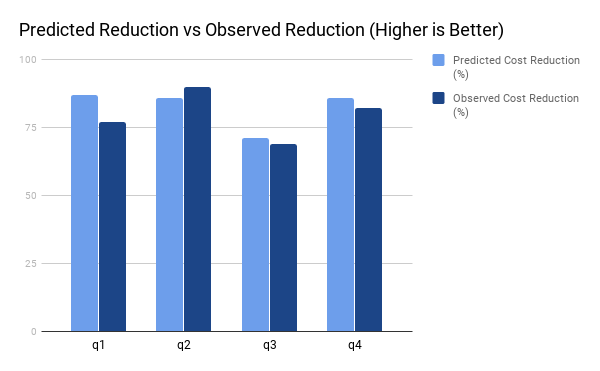
\includegraphics[width=\linewidth]{chart.png}
	%\vspace*{-15pt}
	\caption{Model Based Result: Predicted reduction in cost versus Actual reduction in cost for HIVE on MR queries}
	\label{fig:modelbasedresult}
\end{figure}

We also evaluated effectiveness of the same technique on SparkSQL. Algorithm for it is very similar to $OptResource$ and we are skipping it for brevity. We ran it on 3 real world SparkSQL customer queries. Figure \ref{fig:modelbasedresultspark} shows that the predicted percent reduction in cost matches that of actual reduction is cost observed with very high accuracy.

\begin{figure}[h]
	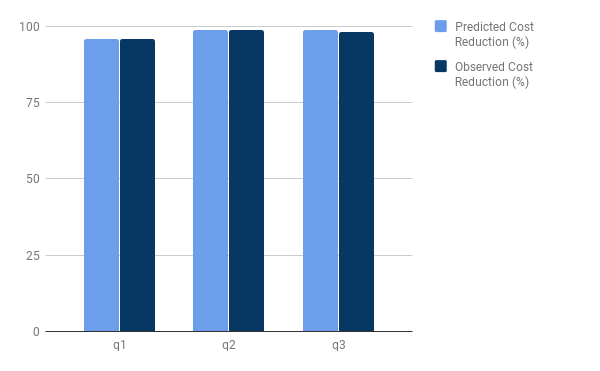
\includegraphics[width=\linewidth]{chart_spark.png}
	%\vspace*{-15pt}
	\caption{Model Based Result: Predicted reduction in cost versus Actual reduction in cost for SparkSQL queries}
	\label{fig:modelbasedresultspark}
\end{figure}
\section{Conclusions}
This paragraph will end the body of this sample document.
Remember that you might still have Acknowledgments or
Appendices; brief samples of these
follow.  There is still the Bibliography to deal with; and
we will make a disclaimer about that here: with the exception
of the reference to the \LaTeX\ book, the citations in
this paper are to articles which have nothing to
do with the present subject and are used as
examples only.
%\end{document}  % This is where a 'short' article might terminate



\appendix
%Appendix A
\section{Headings in Appendices}
The rules about hierarchical headings discussed above for
the body of the article are different in the appendices.
In the \textbf{appendix} environment, the command
\textbf{section} is used to
indicate the start of each Appendix, with alphabetic order
designation (i.e., the first is A, the second B, etc.) and
a title (if you include one).  So, if you need
hierarchical structure
\textit{within} an Appendix, start with \textbf{subsection} as the
highest level. Here is an outline of the body of this
document in Appendix-appropriate form:
\subsection{Introduction}
\subsection{The Body of the Paper}
\subsubsection{Type Changes and  Special Characters}
\subsubsection{Math Equations}
\paragraph{Inline (In-text) Equations}
\paragraph{Display Equations}
\subsubsection{Citations}
\subsubsection{Tables}
\subsubsection{Figures}
\subsubsection{Theorem-like Constructs}
\subsubsection*{A Caveat for the \TeX\ Expert}
\subsection{Conclusions}
\subsection{References}
Generated by bibtex from your \texttt{.bib} file.  Run latex,
then bibtex, then latex twice (to resolve references)
to create the \texttt{.bbl} file.  Insert that \texttt{.bbl}
file into the \texttt{.tex} source file and comment out
the command \texttt{{\char'134}thebibliography}.
% This next section command marks the start of
% Appendix B, and does not continue the present hierarchy
\section{More Help for the Hardy}

Of course, reading the source code is always useful.  The file
\path{acmart.pdf} contains both the user guide and the commented
code.

\begin{acks}
  The authors would like to thank Dr. Yuhua Li for providing the
  matlab code of  the \textit{BEPS} method. 

  The authors would also like to thank the anonymous referees for
  their valuable comments and helpful suggestions. The work is
  supported by the \grantsponsor{GS501100001809}{National Natural
    Science Foundation of
    China}{http://dx.doi.org/10.13039/501100001809} under Grant
  No.:~\grantnum{GS501100001809}{61273304}
  and~\grantnum[http://www.nnsf.cn/youngscientsts]{GS501100001809}{Young
    Scientsts' Support Program}.

\end{acks}
